% Options for packages loaded elsewhere
\PassOptionsToPackage{unicode}{hyperref}
\PassOptionsToPackage{hyphens}{url}
%
\documentclass[11pt]{article}
\usepackage{lmodern}
\usepackage{amssymb,amsmath}
\usepackage[inline]{enumitem}
\usepackage{caption}
\usepackage{ifxetex,ifluatex}
\ifnum 0\ifxetex 1\fi\ifluatex 1\fi=0 % if pdftex
  \usepackage[T1]{fontenc}
  \usepackage[utf8]{inputenc}
  \usepackage{textcomp} % provide euro and other symbols
\else % if luatex or xetex
  \usepackage{unicode-math}
  \defaultfontfeatures{Scale=MatchLowercase}
  \defaultfontfeatures[\rmfamily]{Ligatures=TeX,Scale=1}
\fi
% Use upquote if available, for straight quotes in verbatim environments
\IfFileExists{upquote.sty}{\usepackage{upquote}}{}
\IfFileExists{microtype.sty}{% use microtype if available
  \usepackage[]{microtype}
  \UseMicrotypeSet[protrusion]{basicmath} % disable protrusion for tt fonts
}{}
\makeatletter
\@ifundefined{KOMAClassName}{% if non-KOMA class
  \IfFileExists{parskip.sty}{%
    \usepackage{parskip}
  }{% else
    \setlength{\parindent}{0pt}
    \setlength{\parskip}{6pt plus 2pt minus 1pt}}
}{% if KOMA class
  \KOMAoptions{parskip=half}}
\makeatother
\usepackage{xcolor}
\IfFileExists{xurl.sty}{\usepackage{xurl}}{} % add URL line breaks if available
\IfFileExists{bookmark.sty}{\usepackage{bookmark}}{\usepackage{hyperref}}
\hypersetup{
  hidelinks,
  pdfcreator={LaTeX via pandoc}}
\urlstyle{same} % disable monospaced font for URLs
\usepackage[margin=0.8in]{geometry}
\usepackage{longtable,booktabs}
% Correct order of tables after \paragraph or \subparagraph
\usepackage{etoolbox}
\makeatletter
\patchcmd\longtable{\par}{\if@noskipsec\mbox{}\fi\par}{}{}
\makeatother
% Allow footnotes in longtable head/foot
\IfFileExists{footnotehyper.sty}{\usepackage{footnotehyper}}{\usepackage{footnote}}
\makesavenoteenv{longtable}
\usepackage{graphicx}
\makeatletter
\def\maxwidth{\ifdim\Gin@nat@width>\linewidth\linewidth\else\Gin@nat@width\fi}
\def\maxheight{\ifdim\Gin@nat@height>\textheight\textheight\else\Gin@nat@height\fi}
\makeatother
% Scale images if necessary, so that they will not overflow the page
% margins by default, and it is still possible to overwrite the defaults
% using explicit options in \includegraphics[width, height, ...]{}
\setkeys{Gin}{width=\maxwidth,height=\maxheight,keepaspectratio}
% Set default figure placement to htbp
\makeatletter
\def\fps@figure{htbp}
\makeatother
\setlength{\emergencystretch}{3em} % prevent overfull lines
%\providecommand{}{%
%  \setlength{\itemsep}{0pt}\setlength{\parskip}{0pt}}
\setcounter{secnumdepth}{-\maxdimen} % remove section numbering
\let\oldsection\section
\renewcommand{\section}[1]{\clearpage\oldsection{#1}}
\author{}
\date{}

\begin{document}

\hypertarget{the-ellipse}{%
\section{The Ellipse}\label{the-ellipse}}

The ellipse is, geometrically, a circle that has been stretched in the
\(x\) and/or \(y\) directions. It has useful reflection properties and
is most famous, perhaps, for defining the shape of a closed orbit in a
2-body orbital system.

\textbf{Geometric Definition}: Given two fixed points in a plane,
\(F_1\) and \(F_2\), and a constant \(k > 0\), the ellipse is the locus
of points \(P\) in the same plane such that \(||PF_1| + ||PF_2|| = k\).
The line through \(F_1\) and \(F_2\) is the \emph{major axis} of the
ellipse. The two points \(F_1,F_2\) are the \emph{foci} (singular:
\emph{focus}) of the ellipse. The \emph{minor axis} is perpendicular to
the major axis. The 4 points at which the ellipse intersects an axis are
the vertices.

\begin{table}[ht]
	\centering
	\begin{tabular}{cc}
		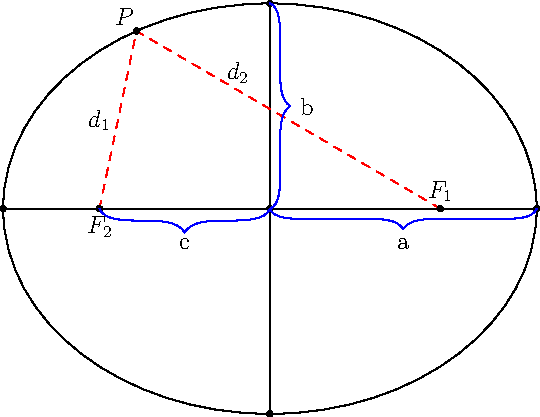
\includegraphics[width=\textwidth,height=2in]{ellipse-schematic.pdf} &
		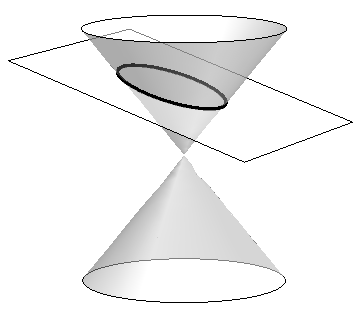
\includegraphics[width=\textwidth,height=2in]{conic_ellipse.png}
	\end{tabular}
	\caption*{A ``wide'' ellipse schematic, and an ellipse in a cone}
\end{table}

\textbf{Parent Equation}:
  \begin{itemize}
		\item \(\dfrac{x^2}{a^2}+\dfrac{y^2}{b^2}=1\) is the
equation for a ``wide'' ellipse centered at the origin and
    \item \(\displaystyle \dfrac{x^2}{b^2}+\dfrac{y^2}{a^2}=1\) is the
   equation for a ``tall'' ellipse centered at the origin.
	\end{itemize}
Yes, they are the same,
it's just we have a habit of associating $a$ with the larger denominator.
The semi-major axis
length is $a$ and the semi-minor axis length is $b$.
(The major and minor axis lengths are twice the semi-major axis and
semi-minor axis lengths.)

\textbf{General Equation}:
\begin{itemize}
  \item \(\dfrac{(x-h)^2}{a^2} + \dfrac{(y-k)^2}{b^2} = 1\) is a wide ellipse
centered at \((h,k)\).
  \item \(\dfrac{(x-h)^2}{b^2} + \dfrac{(y-k)^2}{a^2} = 1\) is a tall ellipse
  centered at \((h,k)\).
\end{itemize}
\textbf{Properties}

\begin{itemize}

\item
  Length of axes are \(2a\) and \(2b\). The longer one, $2a$, is the major
  axis.
\item
  The distance from the center of the ellipse to either focus is \(c\)
  where \(c^2 = a^2-b^2\).
\item
  The sum of the distances from any point to both foci is the length of the
	major axis.
\item
  The eccentricity of an ellipse is defined as \(e = \dfrac{c}{a}\). A larger eccentricity
	means a more ``stretched'' ellipse.
\item
  The area of an ellipse is \(\pi a b\).
\item
  The perimeter of an ellipse is very complicated.\footnote{If you really
    want to know, it's the value of the ``complete elliptic integral of
    the second kind''
    \(4a \int_0^{\pi/2} \sqrt{1 - e^2 \sin^2 \theta} \; d\theta\), which
    can be approximated by the series
    \(p = \pi(a+b)\left(1 + \frac14 h + \frac{1}{64}h^2 + \frac{1}{256}h^3 + \ldots\right)\)
    where \(h = \frac{(a-b)^2}{(a+b)^2}\)}
\item
  Any ray of light or sound which emanates from one focus will reflect
  to the other focus. You may have experienced this in the US Capitol's
  Whispering Gallery.
\end{itemize}

\textbf{Relation to a circle}. A circle is an ellipse with \(a=b\).

\hypertarget{problems}{%
\subsection{Problems}\label{problems}}

Unless otherwise specified, any ellipse equations should be given in
standard form

\hypertarget{fundamental-concepts}{%
\paragraph{Fundamental Concepts}\label{fundamental-concepts}}

\begin{enumerate}
\def\labelenumi{\arabic{enumi}.}

\item Match the following equations
\vspace{0ex} \\

	\begin{enumerate*}[label=\itshape\Alph*\upshape)]
		\item
			\(\dfrac{x^2}{4}+\dfrac{y^2}{9} = 1\)\hspace{3ex}
		\item
			\(\dfrac{x^2}{9}+\dfrac{y^2}{4} = 1\)\hspace{3ex}
		\item
			\(\dfrac{(x-2)^2}{16} + (y+1)^2 = 1\)\hspace{3ex}
		\item
			\(\dfrac{(x+2)^2}{9}+\dfrac{(y+2)^2}{4} = 1\)
		\end{enumerate*}
		\\

	with the graphs below
	\vspace{0ex}\\

	\begin{enumerate*} [label=\roman*\upshape)]
		\item \includegraphics*[width=1.5in]{pD.pdf}
		\item \includegraphics*[width=1.5in]{pA.pdf}
		\item \includegraphics*[width=1.5in]{pC.pdf}
		\item \includegraphics*[width=1.5in]{pB.pdf}
	\end{enumerate*}
	\vspace{1ex}\\

\item
  For each of the following problems, find an equation of an ellipse in standard form

  \begin{enumerate}

  \item
    Major axis of length 12, minor axis of length 6
  \item
    Passes through the points \((0,6)\) and \((3,0)\)
  \item
    Foci: \((\pm 4,0)\), major axis 10
  \item
    Vertices: \((\pm 7,0)\), foci: \((\pm 2,0)\)
  \item
    Vertices: \((0, \pm 8)\), foci: \((0, \pm 4)\)
  \end{enumerate}
\item
  For each of the following problems, find an equation of an ellipse in standard form
  \begin{enumerate}

  \item
    Vertices: \((2,0), (10,0)\); minor axis length 4
  \item
    Foci: \((0,0), (4,0)\), major axis length 6
  \item
    Center: \((2,-1)\), vertex \((2,\frac12)\),minor axis length 2
  \end{enumerate}
\item
  Find the center, vertices, foci, eccentricity and sketch each of the following

  \begin{enumerate}

  \item
    \(\dfrac{x^2}{25} + \dfrac{y^2}{16} = 1\)
  \item
    \(\dfrac{x^2}{16} + \dfrac{y^2}{81} = 1\)
  \item
    \(\dfrac{(x-4)^2}{16} + \dfrac{(y+1)^2}{25} = 1\)
  \item
    \(\dfrac{(x-5)^2}{9/4} + (y-1)^2 = 1\)
  \item
    \(9x^2 + 4y^2 + 36x - 24y + 36 = 0\)
  \item
    \(12x^2 + 20y^2 - 12x + 40y - 37 = 0\)
  \end{enumerate}
\item
  Find the equation of an ellipse with vertices \((\pm 5,0)\) and
  eccentricity \(e = \dfrac{4}{5}\).

\end{enumerate}

\hypertarget{deeper-understanding}{%
\paragraph{Deeper Understanding}\label{deeper-understanding}}

\begin{enumerate}
\def\labelenumi{\arabic{enumi}.}
\setcounter{enumi}{5}

\item
  \textbf{Echo Chamber.} Statuary Hall is an elliptical room in the United States Capitol in
  Washington, D.C. The room is also called the Whispering Gallery
  because a person standing at one focus of the room can hear even a
  whisper spoken by a person standing at the other focus. The dimensions
  of Statuary Hall are 46 feet wide by 97 feet long.

  \begin{enumerate}

  \item
    Find an equation of the shape of the room.
  \item
    Determine the distance between the foci.
  \end{enumerate}
\item
  \textbf{Artificial Satellites.} The first artificial satellite to orbit Earth was Sputnik I (launched
  by the former Soviet Union in 1957). Its highest point above Earth's
  surface was 939 kilometers, and its lowest point was 215 kilometers
  (see figure). The center of Earth was at one focus of the elliptical
  orbit. Find the eccentricity of the orbit. (Assume the radius of Earth
  is 6378 kilometers.)
\item
  \textbf{Ellipse geometry.}
	Find an equation of an ellipse such that for any point \(P\) on the
  ellipse, the sum of the distances from the point \(P\) to the points
  \((2, 2)\) and \((10, 2)\) is 36.
\item
	\textbf{Thinking outside the ellipse.}
  How many ellipses centered at the origin contain the points \((1,1)\)
  and \((1,-1)\)? Describe all the solutions.
\item
	\textbf{Eccentricities.}
	What is the domain of $e$? That is, what values can the eccentricity of an ellipse assume?
\item
  \textbf{Infinite limits.}
	Write the formula for eccentricity using only \(a\) and \(b\). Analyze
  the limits as \(a \to b\) and as \(a \to \infty\).
\item
  \textbf{Orbital mechanics.}
  \begin{enumerate}
  \item
    The Earth orbits the sun in an (approximately\footnote{It would be a
      perfect ellipse if it weren't for the moon, and Jupiter and, to a
      much smaller extent, all the other planets.}) elliptical orbit
    with the Sun at one focus. This is Kepler's Law. The average distance from
    the sun to the Earth is defined as one astronomical units (AU).
    Since the distance to the sun varies over one year, there is a point in its orbit
		where the earth is
    closest to the sun (perihelion) and and a point where it is furthest (aphelion).
  \item
    Using a reliable resource, determine the values of the distances at
    aphelion and perihelion for the Earth in AU. Also look up the eccentricity of the
		Earth's elliptical orbit.
  \item
    Using these values, write the equation of the Earth's orbit in
    standard form, where \(x\) and \(y\) are measured in units of AU.
    Assume the Sun is at a focus and positioned to the right of the center of the
    ellipse, on the \(x\)-axis.
  \end{enumerate}
\item
  \textbf{Shared focus.}
	Confocal ellipses have the same foci. Show that, for \(k>0\), all
  ellipses of the form \(\dfrac{x^2}{6+k}+\dfrac{y^2}{k}=1\) are
  confocal.
\item
  \textbf{Square in an ellipse.}
	A square is inscribed inside an ellipse with major axis length 5 and
  minor axis length 4. What is the area of the square? (\emph{Inscribed}
  means the vertices of the square are on the ellipse).
\item
	\textbf{Reflection properties}
	An elliptical pool table would send a ball from one focus straight to the other focus, regardless
	of where the ball is hit. This is because the angle of incidence and the angle of reflection
	on the boundary of an ellipse are always the same. This problem explores that geometric property.

	The ellipse \(E\) has vertices at \((\pm 6,0)\) and \((0, \pm 4)\).

	\begin{enumerate}
	\item
  The line \(y=4\) is tangent to the ellipse at point \(P = (0,4)\). The
  angles \(\alpha\) and \(\beta\) are the same in Figure 3. Find
  \(\alpha\). \\
	\begin{center}
		\includegraphics*[width=2.75in]{ellipse2.pdf}
	\end{center}

  \item
    Let
    \(P\) be the point on \(E\) in the first quadrant with
    \(x\)-coordinate 2. The tangent line at \(P\) also makes equivalent
    angles with the lines from \(P\) to the two foci. Find the equation
    of the tangent line.
		\begin{center}
			\includegraphics*[width=2.75in]{ellipse3.pdf}
		\end{center}
  \item
    Find the coordinate in the first quadrant at which the tangent line
    makes a \(30^\circ\) angle with the lines to the foci.
  \item
    What is the maximum angle the tangent line makes with the lines to
    the foci?
  \end{enumerate}

\item
  \textbf{Derivations and proofs.}
	Derive the parent equation of an ellipse from its geometric
  definition (the sum of the distances from a point to the foci is constant).
\end{enumerate}

\end{document}
